\section{Introduction}
Approximate Nearest Neighbor Search (ANNS) is a core primitive in modern data systems, including Retrieval-Augmented Generation (RAG), recommendation, and anomaly detection~\cite{Zhong20255017}. Graph-based indices such as HNSW~\cite{Jayaram2019, Malkov2020824} are widely adopted because they offer strong recall-latency trade-offs at scale. Their search process relies on graph traversal over non-contiguous memory regions, where random access and cache misses often dominate runtime. Existing acceleration techniques generally follow two directions: system-level optimizations that compute faster (e.g., layout, SIMD, quantization)~\cite{Gou2025, Wang2025, Zhong20255017}, and algorithm-level optimizations that compute less (e.g., pruning and distance estimation)~\cite{Chen20233225, Gao2023, Song2025}.

Despite substantial progress, most optimizations are developed for static or slowly evolving data snapshots. In practical streaming systems, vectors are continuously inserted and deleted, creating a temporal mismatch: auxiliary search metadata that is effective at time $t$ may become stale at time $t+\Delta$. This mismatch is particularly pronounced in high-rate pipelines (e.g., social-content ingestion), where distribution shift and index-topology evolution occur concurrently.

This setting induces a fundamental efficiency-maintenance dilemma, illustrated in Figure~\ref{fig:motivation}. Without maintenance, query throughput (QPS) degrades as optimization hints lose validity (Figure~\ref{fig:stale-hint}); with frequent global re-optimization, maintenance overhead dominates end-to-end cost (Figure~\ref{fig:reopt-cost}). Consequently, the key challenge is not merely how to accelerate search, but how to keep acceleration \emph{continuously valid} under ongoing updates.

\begin{figure}
	\centering
	\subfloat[Staleness-induced performance decay]{
		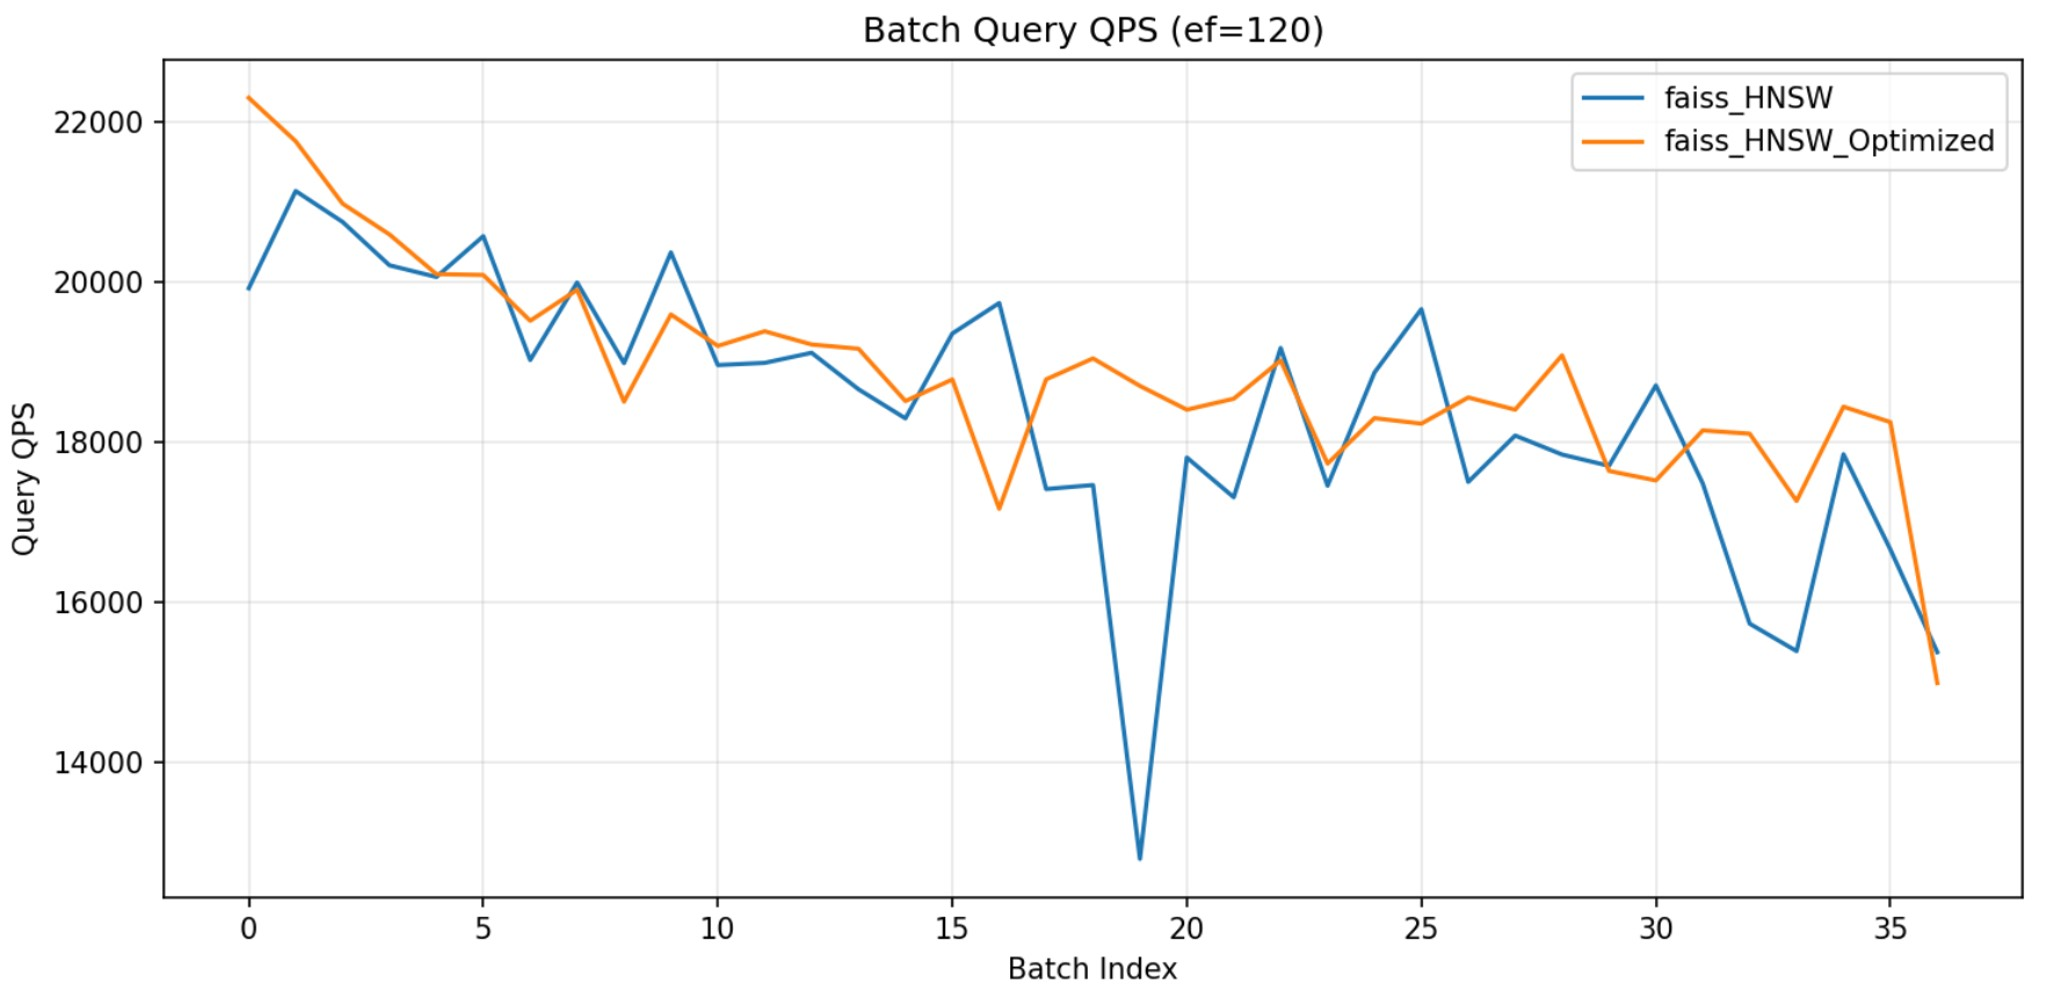
\includegraphics[width=\columnwidth]{figures/figure1a.jpg}
		\label{fig:stale-hint}
	}
    \\
    \subfloat[Cost of frequent global re-optimization]{
		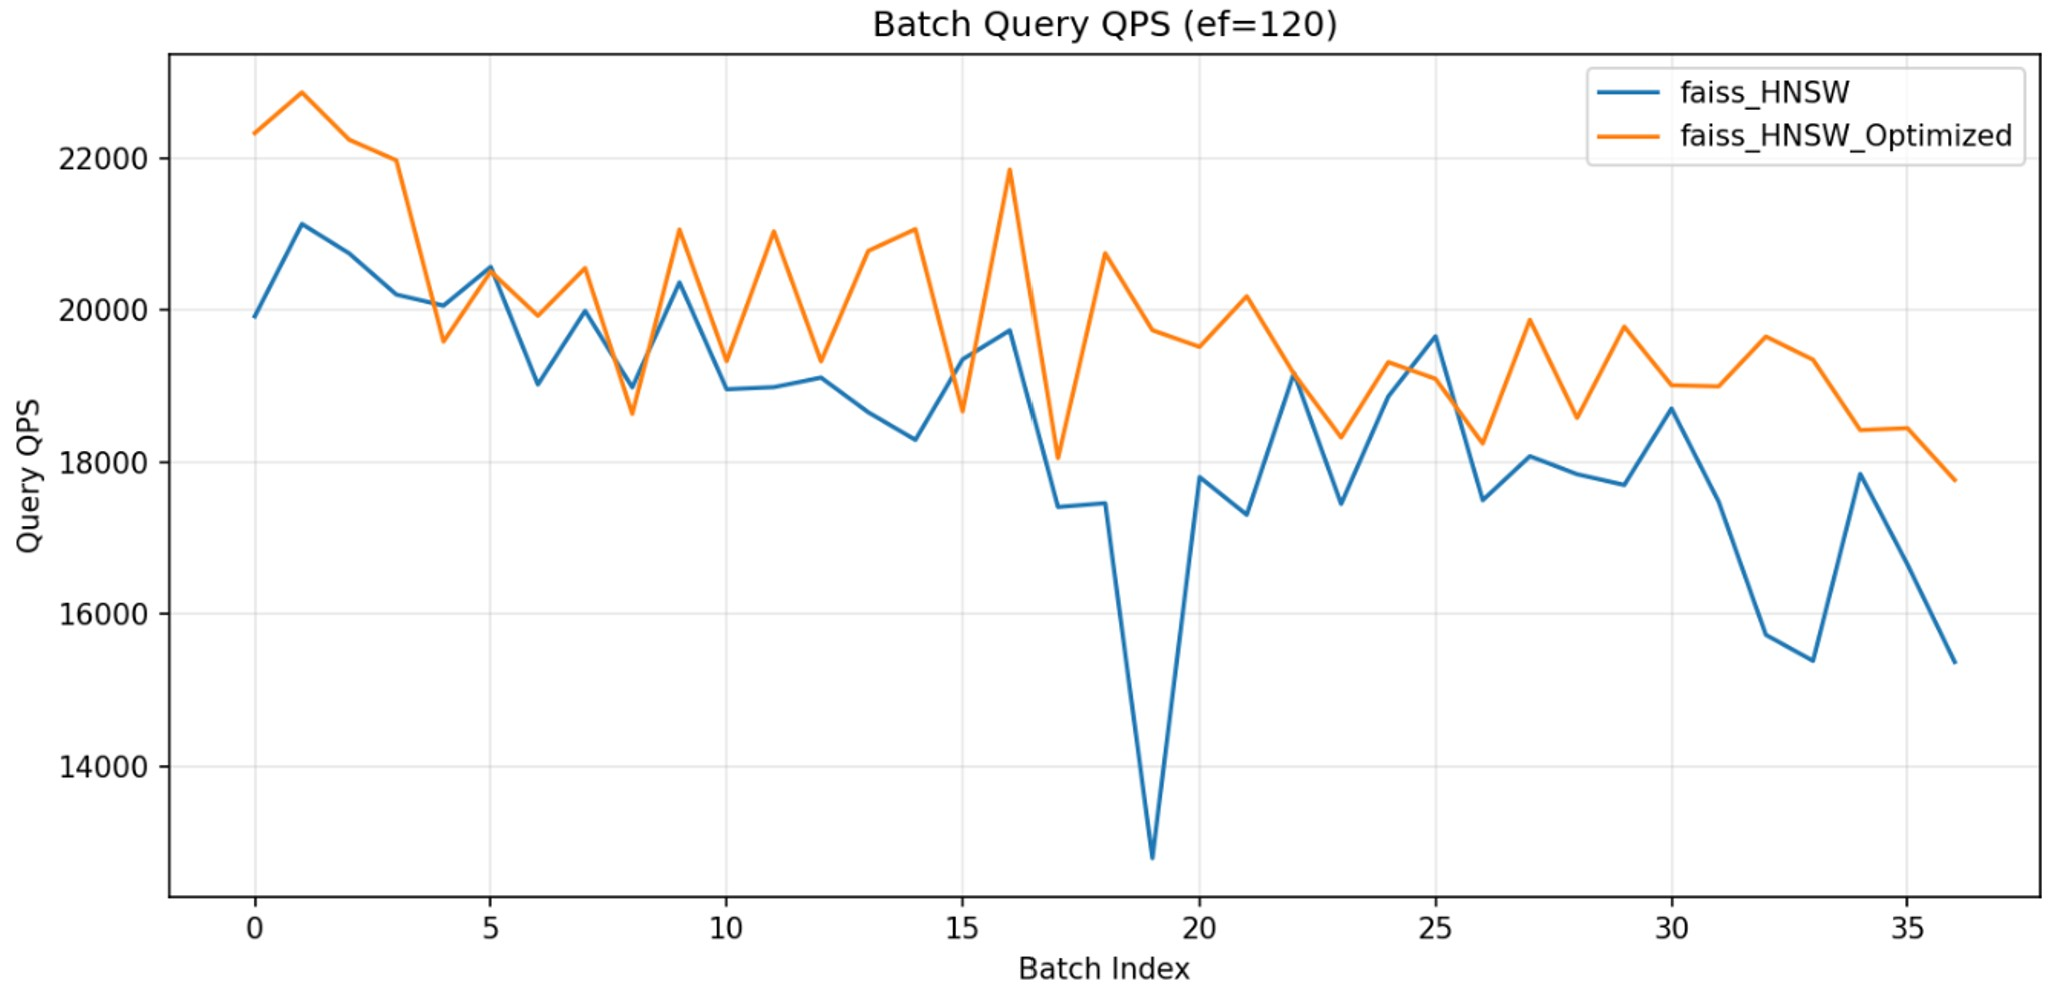
\includegraphics[width=\columnwidth]{figures/figure1b.jpg}
		\label{fig:reopt-cost}
	}
    \caption{Motivating trade-off in dynamic ANNS: stale hints hurt search efficiency, while aggressive global maintenance hurts amortized throughput.}
	\label{fig:motivation}
\end{figure}

\noindent\textbf{Key idea and design overview.}
Rather than optimizing static snapshots, StreamSeed formulates acceleration as an online control problem under drift.
The design is organized around two aspects.
\textbf{Design Aspect I (Workload-aligned reuse under drift)} renders hint reuse selective and self-correcting: reuse is enabled when recent evidence indicates positive utility and disabled when confidence degrades.
\textbf{Design Aspect II (Backend-decoupled control interface)} separates policy logic from backend mechanics, enabling a shared policy family to be reused across dynamic ANN backends with low integration overhead.

\noindent\textbf{Contributions.}
This paper makes the following contributions:
\begin{itemize}
	\item We formalize the stale-hint problem in streaming ANNS as an amortized search-maintenance optimization problem, clarifying why static accelerations degrade in dynamic regimes.
	\item We present StreamSeed with two explicit design aspects: workload-aligned reuse under drift and a backend-decoupled control interface.
	\item We implement StreamSeed in CANDOR-Bench through a pluginized policy--adapter--runtime structure and runbook-driven configuration, enabling reproducible dynamic evaluations across workloads.
	\item We provide empirical results and ablations showing that unified query-hint control improves end-to-end efficiency while maintaining competitive recall under high update rates.
\end{itemize}

\noindent\textbf{Paper organization.}
Section 2 formalizes the problem and preliminaries.
Section 3 presents the StreamSeed design.
Section 4 describes implementation details in CANDOR-Bench.
Section 5 reports evaluation and ablation results.
Section 6 discusses related work, and Section 7 concludes.
